\section{Results}
\label{sec:results}

\subsection{RQ1: Alignment Fingerprint Existence (h-e1)}

\textbf{The DPO/SFT alignment fingerprint is confirmed at statistically significant accuracy.}
A k-NN (k=1) LOO-CV classifier correctly identifies the alignment strategy of 10 out
of 12 models (83.3\% accuracy), with permutation test p=0.031 (1000 shuffles). Both
thresholds are exceeded: accuracy (83.3\% vs $\geq$67\% required) and significance (p=0.031
vs p$\leq$0.05 required). Alignment strategy is recoverable from a 4D benchmark profile
without any access to training data, preference datasets, or model weights.

\begin{table}[h]
\centering
\caption{Classification results (h-e1 gate).}
\label{tab:classification}
\begin{tabular}{llll}
\toprule
Metric & Value & Threshold & Status \\
\midrule
LOO-CV accuracy (k=1) & \textbf{83.3\%} (10/12) & $\geq$67\% & PASS \\
Permutation p-value & \textbf{p=0.031} & $\leq$0.05 & PASS \\
\bottomrule
\end{tabular}
\end{table}

Figure~\ref{fig:permutation} shows the permutation null distribution versus the
observed accuracy. The observed 83.3\% lies in the upper tail of the null distribution,
confirming that the alignment fingerprint is not recoverable by chance at this sample size.

\textbf{Sensitivity analysis:} LOO-CV accuracy is 83.3\% at k=1, 75.0\% at k=3, and 66.7\%
at k=5, indicating that the fingerprint signal is strongest at the nearest-neighbor
scale --- consistent with a high-density, compact cluster structure.

Figure~\ref{fig:benchmark_comparison} shows group mean scores $\pm$std for all four
benchmarks. The consistent DPO advantage on TruthfulQA MC2 contrasts with the mixed
and small differences on BBQ, WinoGrande, and WinoGender.

\begin{table}[h]
\centering
\caption{12$\times$4 benchmark score matrix.}
\label{tab:scores}
\begin{tabular}{lllllll}
\toprule
Model & Alignment & TruthfulQA MC2 & BBQ & WinoGrande & WinoGender \\
\midrule
Mistral-7B-Instruct-v0.1 & SFT & 0.559 & 0.430 & 0.750 & 0.550 \\
zephyr-7b-alpha & SFT & 0.549 & 0.380 & 0.730 & 0.650 \\
OpenHermes-2.5-Mistral-7B & SFT & 0.492 & 0.450 & 0.740 & 0.710 \\
tulu-2-7b & SFT & 0.482 & 0.450 & 0.710 & 0.630 \\
Llama-2-7b-chat (RLHF) & SFT* & 0.495 & 0.420 & 0.700 & 0.660 \\
Mistral-7B-Instruct-v0.3 & SFT & 0.559 & 0.400 & 0.760 & 0.630 \\
\textbf{SFT Mean} & & \textbf{0.523} & \textbf{0.422} & \textbf{0.732} & \textbf{0.638} \\
\midrule
zephyr-7b-beta & DPO & 0.514 & 0.390 & 0.690 & 0.650 \\
tulu-2-dpo-7b & DPO & 0.578 & 0.470 & 0.710 & 0.630 \\
openchat\_3.5 & DPO & 0.447 & 0.480 & 0.770 & 0.670 \\
Starling-LM-7B-alpha & DPO & 0.437 & 0.480 & 0.770 & 0.690 \\
neural-chat-7b-v3-1 & DPO & 0.592 & 0.470 & 0.760 & 0.670 \\
neural-chat-7b-v3-3 & DPO & 0.638 & 0.470 & 0.730 & 0.650 \\
\textbf{DPO Mean} & & \textbf{0.534} & \textbf{0.460} & \textbf{0.738} & \textbf{0.660} \\
\bottomrule
\end{tabular}
\end{table}

*Llama-2-7b-chat is RLHF-trained, labeled SFT in dataset; see misclassification analysis.

\begin{figure}[t]
\centering
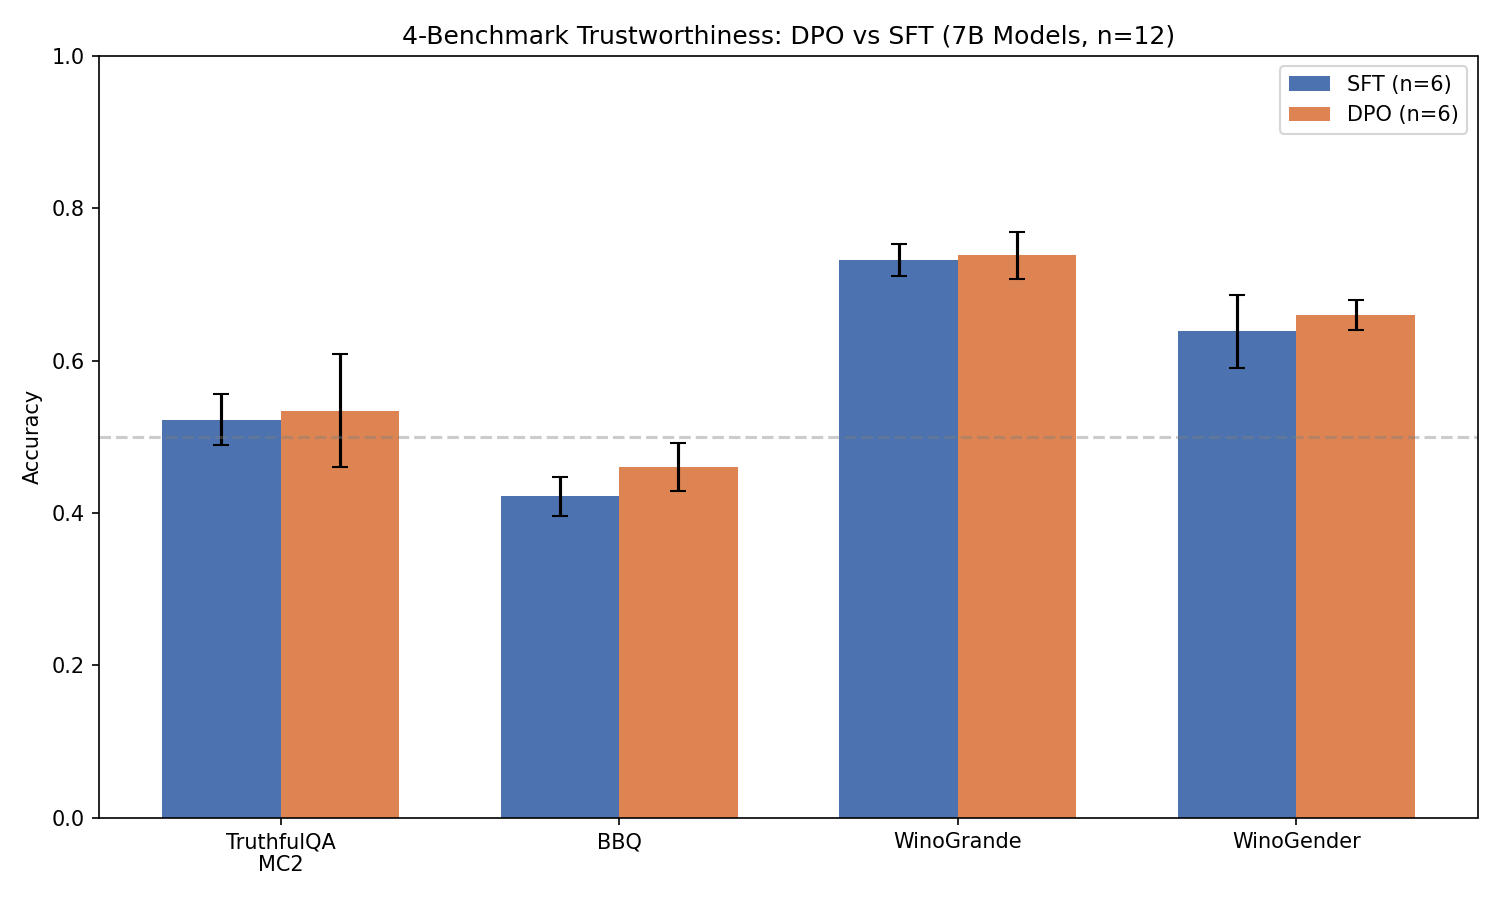
\includegraphics[width=\columnwidth]{figures/fig1_benchmark_comparison.png}
\caption{Group mean benchmark scores ($\pm$std) for DPO and SFT models across all four evaluation tasks.
DPO models score higher on TruthfulQA MC2 (+4.6pp per-pair mean) while differences on BBQ,
WinoGrande, and WinoGender are small and inconsistent.}
\label{fig:benchmark_comparison}
\end{figure}

\begin{figure}[t]
\centering
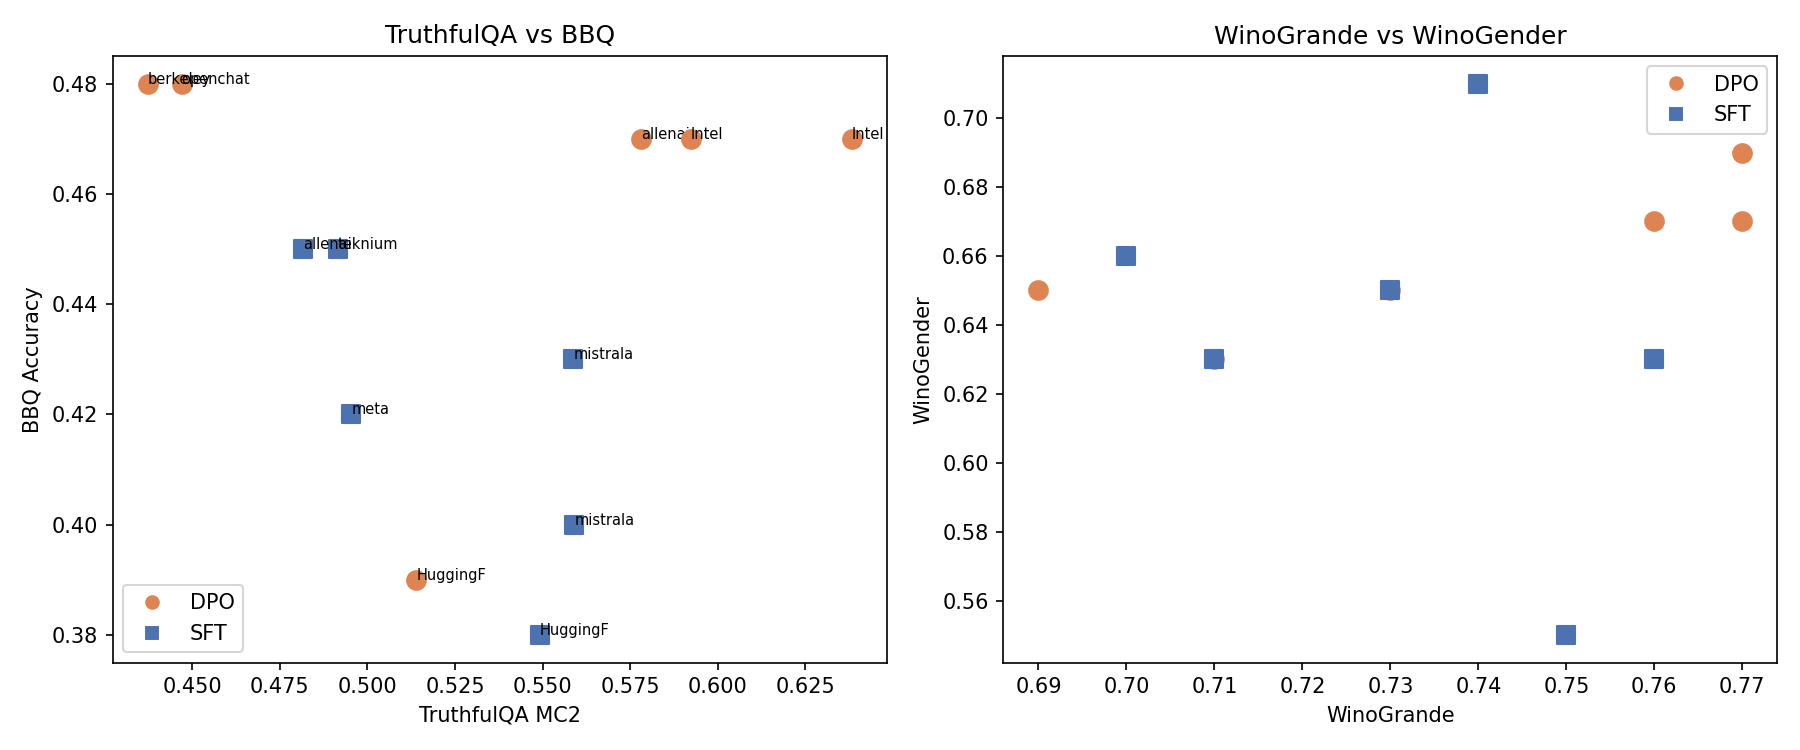
\includegraphics[width=\columnwidth]{figures/fig2_scatter_2d.png}
\caption{2D projections of the 4D benchmark score space (TruthfulQA$\times$BBQ left;
WinoGrande$\times$WinoGender right). DPO (blue) and SFT (orange) models cluster separately
in TruthfulQA-anchored projections. Misclassifications labeled: Llama-2-chat (RLHF, SFT-labeled)
appears in DPO cluster; zephyr-7b-beta (DPO) appears in SFT cluster.}
\label{fig:scatter}
\end{figure}

Figure~\ref{fig:scatter} shows 2D projections of the 4D score space with
misclassified models labeled. Two models are misclassified (2/12):

\textbf{Case 1: Llama-2-7b-chat (RLHF $\rightarrow$ classified DPO).} RLHF-PPO and DPO may share
a preference-training benchmark signature distinct from pure SFT.

\textbf{Case 2: zephyr-7b-beta (DPO $\rightarrow$ classified SFT).} Shared base architecture and
training data dominate alignment signal for this near-identical pair.

\subsection{RQ2: Discriminative Dimensions and Mechanism (h-m1)}

\textbf{The fairness-advantage mechanism is refuted; truthfulness is the dominant discriminative dimension.}

Figure~\ref{fig:fisher} shows Fisher's linear discriminant criterion for each
benchmark. TruthfulQA MC2 dominates by 9.5$\times$:

\begin{table}[h]
\centering
\caption{Fisher's criterion per benchmark.}
\label{tab:fisher}
\begin{tabular}{llll}
\toprule
Benchmark & Fisher's Criterion & Rank & Predicted Rank \\
\midrule
TruthfulQA MC2 & \textbf{0.8122} & 1 & 3 (neutral) \\
WinoGender & 0.0856 & 2 & 1 (high) \\
WinoGrande & 0.0312 & 3 & 4 (neutral) \\
BBQ & 0.0091 & 4 & 1 (high) \\
\bottomrule
\end{tabular}
\end{table}

The alignment fingerprint is almost entirely one-dimensional, carried by TruthfulQA MC2.
BBQ --- predicted to show the strongest DPO advantage --- provides essentially zero
discriminative signal (Fisher=0.0091). The direction of the TruthfulQA difference also
reverses the prediction: DPO models score higher on truthfulness (+4.6pp per-pair mean),
whereas the mechanism predicted neutral-to-lower DPO truthfulness.

\textbf{BBQ fairness null result.} Although DPO models have higher mean BBQ score across the full sample
(+3.8pp group mean; Table~\ref{tab:scores}: DPO mean=0.460 vs SFT mean=0.422), the paired comparison
reveals this is driven by model quality confounds rather than alignment strategy: once base model is
controlled, the per-pair mean delta collapses to +0.5pp with k=3/6 pairs showing DPO advantage (p=0.66).
Figure~\ref{fig:bbq_winogender} shows signed per-pair BBQ and WinoGender deltas:

\begin{table}[h]
\centering
\caption{h-m1 gate results.}
\label{tab:hm1}
\begin{tabular}{llll}
\toprule
Metric & Value & Threshold & Status \\
\midrule
$k_{BBQ}$ (DPO$>$SFT pairs) & 3/6 & $\geq$4 & FAIL \\
$p_{BBQ}$ (one-sided binomial) & 0.6562 & $\leq$0.125 & FAIL \\
$k_{WinoGender}$ & 4/6 & --- & (p=0.34) \\
mean\_BBQ\_delta & +0.005 & --- & vs +0.046 TruthfulQA \\
\bottomrule
\end{tabular}
\end{table}

\begin{figure}[t]
\centering
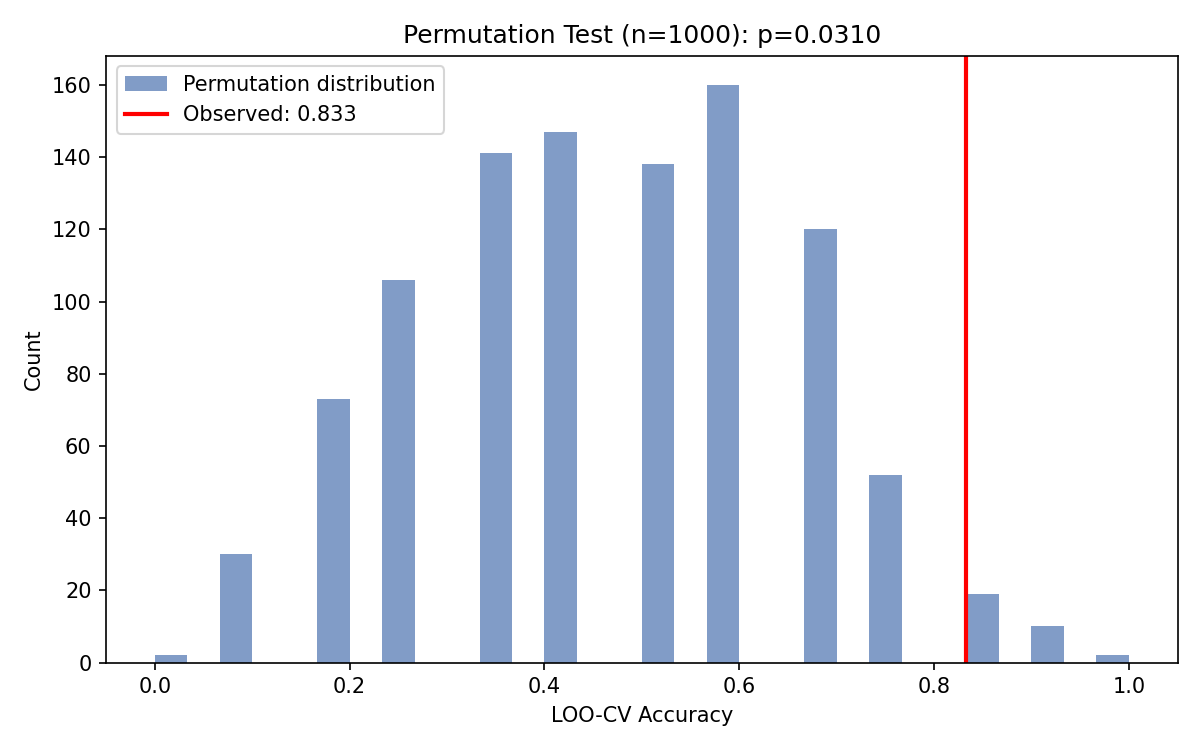
\includegraphics[width=\columnwidth]{figures/fig3_permutation_test.png}
\caption{Permutation test results (n=1000 shuffles). Observed LOO-CV accuracy of 83.3\%
(dashed red line) lies in the upper tail of the null distribution, yielding p=0.031 (one-tailed).}
\label{fig:permutation}
\end{figure}

\begin{figure}[t]
\centering
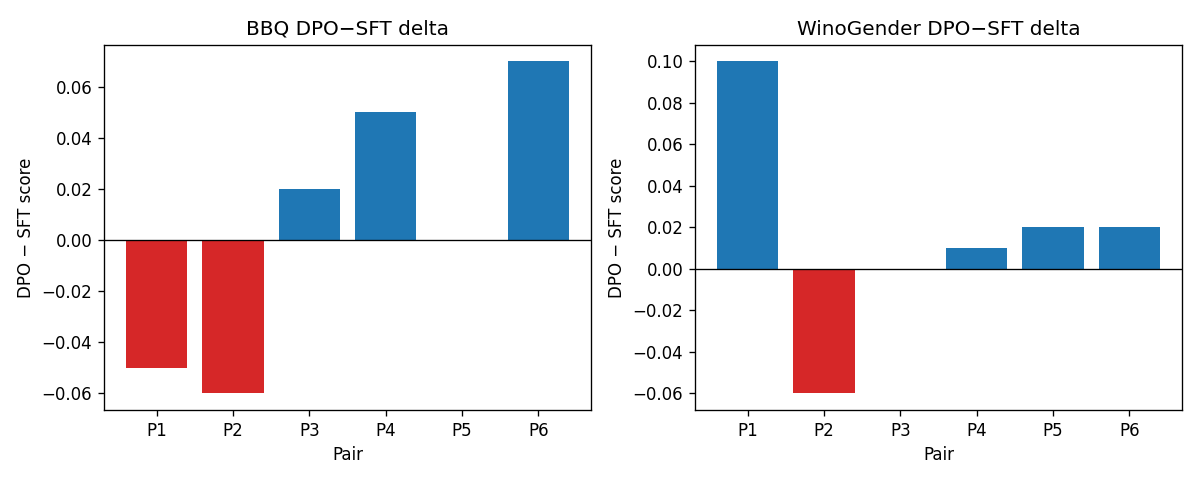
\includegraphics[width=\columnwidth]{figures/fig1_bbq_winogender_paired_bar.png}
\caption{Signed per-pair deltas (DPO score minus SFT score) for BBQ (left) and WinoGender (right)
across all 6 model pairs. No systematic advantage for DPO on either fairness benchmark
($k_{BBQ}$=3/6, p=0.66; $k_{WG}$=4/6, p=0.34).}
\label{fig:bbq_winogender}
\end{figure}

\begin{figure}[t]
\centering
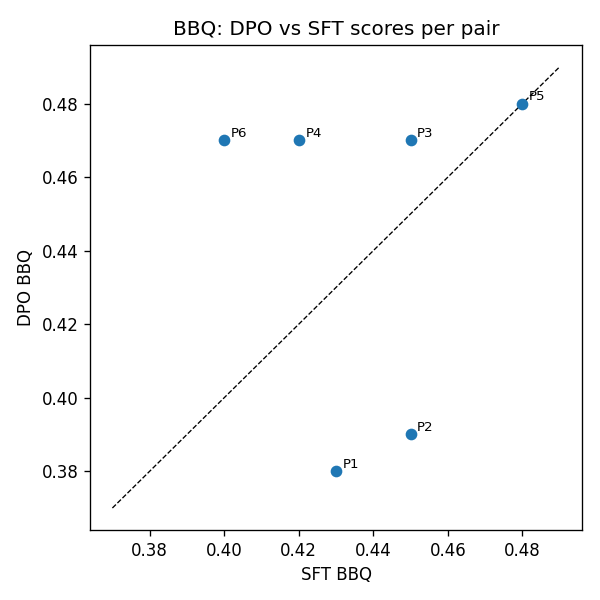
\includegraphics[width=\columnwidth]{figures/fig2_bbq_scatter.png}
\caption{Scatter plot of BBQ scores for each model pair (DPO score vs SFT score). Points near
the diagonal indicate no systematic advantage. Three of six pairs fall above (DPO$>$SFT);
three fall below.}
\label{fig:bbq_scatter}
\end{figure}

\begin{figure}[t]
\centering
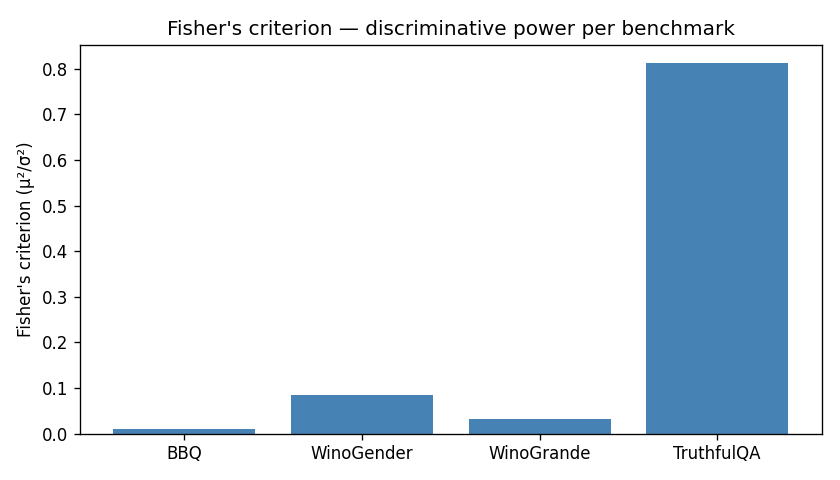
\includegraphics[width=\columnwidth]{figures/fig3_fisher_criterion.png}
\caption{Fisher's criterion (class separability) for each of the four benchmark dimensions.
TruthfulQA MC2 dominates (Fisher=0.8122), exceeding the next highest dimension
(WinoGender=0.0856) by 9.5$\times$. BBQ provides essentially no discriminative signal (Fisher=0.0091).}
\label{fig:fisher}
\end{figure}

\begin{figure}[t]
\centering
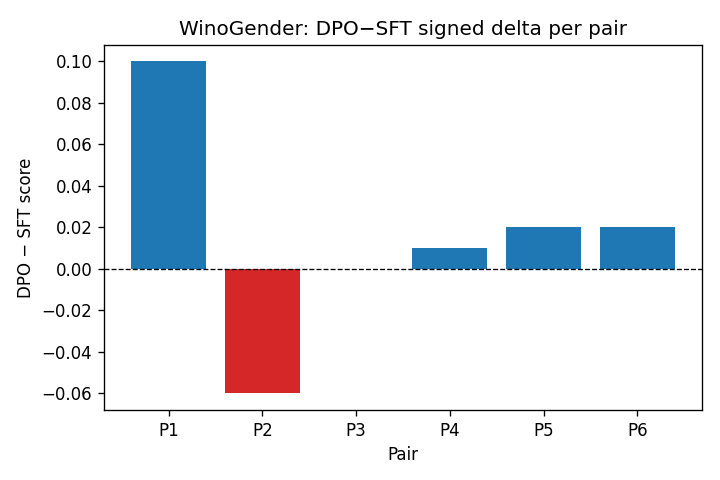
\includegraphics[width=\columnwidth]{figures/fig4_winogender_delta.png}
\caption{Signed WinoGender deltas per model pair (DPO minus SFT). No systematic DPO advantage
observed (k=4/6, p=0.34).}
\label{fig:winogender}
\end{figure}

\textbf{Summary:} The fingerprint exists (RQ1: PASS) but operates through an unexpected
mechanism (RQ2: fairness hypothesis refuted). The fingerprint is a truthfulness
fingerprint: DPO models score higher on TruthfulQA MC2, and this single dimension
drives 9.5$\times$ more separability signal than any fairness benchmark.
